\documentclass[10pt]{article}
\usepackage{amsmath}
\usepackage{amssymb}
\usepackage{graphicx}
\usepackage{hyperref}
\usepackage[latin1]{inputenc}
\usepackage{listings}
\usepackage{pgfplots}
\usepackage{hyperref}
\usepackage{geometry}
\renewcommand{\labelitemi}{$\textendash$}
\renewcommand{\arraystretch}{1.4}
\hypersetup{colorlinks=true, urlcolor=cyan}
\geometry{
    a4paper,
    total={170mm,257mm},
    left=15mm,
    right=15mm,
    top=15mm,
    bottom=15mm
}

\title{\vspace{-5ex}ST3009: Final Assignment\vspace{-2.5ex}}
\author{Conor McCauley - 17323203}
\date{\vspace{-2ex}May 7, 2020\vspace{-2ex}}

\begin{document}

\maketitle

\section*{Question 1}

\noindent (a) There are ${10 \choose 3} = 120$ ways to select 3 distinct topics out of the 10 regardless of order.

\noindent (b) There are $10 - n$ topics remaining that can come up and we can choose 3 of those. Therefore, of the 120 total selections ${10 - n \choose 3}$ of those will not contain any of the $n$ topics. Thus, the probability that none of the studied topics come up is:

$$\frac{{10 - n \choose 3}}{120}$$

\noindent (c) The probability that fewer than 2 studied topics come up is the sum of the probability that exactly 1 studied topic comes up and the probability that no studied topics come up. We already know the probability that no studied topics come up from the previous question. For 1 studied topic, there are ${10 - n \choose 2}$ ways to select the 2 non-studied topics and ${n \choose 1} = n$ ways to select the 1 studied topic. Therefore, the total probability that fewer than 2 studied topics come up is:

$$\frac{{10 - n \choose 3} + {{10 - n \choose 2} \cdot n}}{120}$$

We can plot this probability against $n$ like so:

\begin{center}
    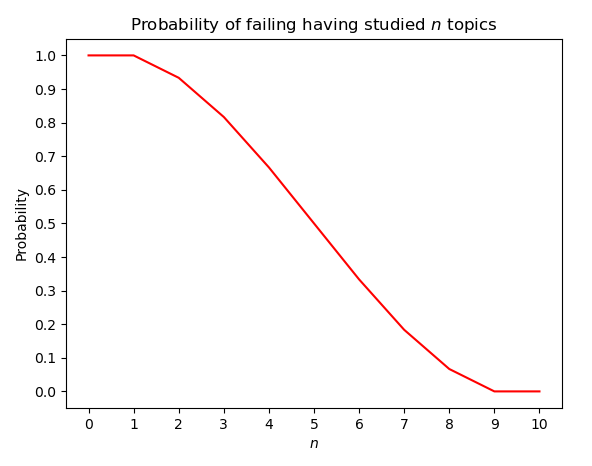
\includegraphics[scale=0.5]{q1_c.png}
\end{center}

\noindent (d) There are ${10 \choose 4} = 210$ ways to select 4 topics for the test. As in part (c), in order for you to fail, fewer than 2 studied topics must come up. There are ${10 - n \choose 4}$ ways to select 4 topics so that none of the $n$ studied topics come up. For 1 studied topic, there are ${10 - n \choose 3}$ ways to select the 3 non-studied topics and ${n \choose 1} = n$ ways to select the 1 studied topic. Therefore, the total probability that fewer than 2 studied topics come up is:

$$\frac{{10 - n \choose 4} + {{10 - n \choose 3} \cdot n}}{210}$$

Again, we can plot this like so:

\begin{center}
    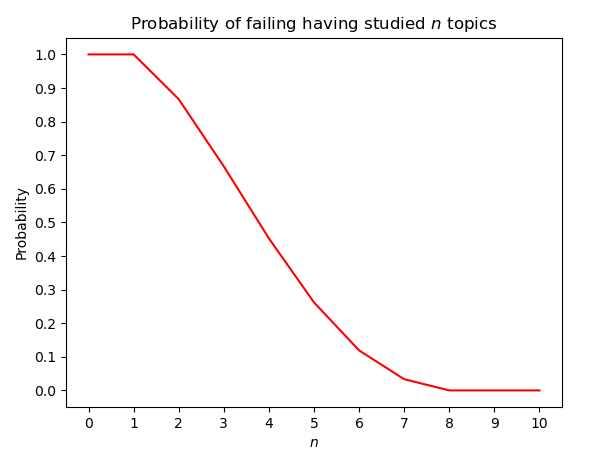
\includegraphics[scale=0.5]{q1_d.png}
\end{center}

As expected, the probability of failing is lower for each value of $n$ as there are more topics on each test while the same number of studied topics are needed to pass the test.

\noindent (e) The pseudo-code of the simulation, \texttt{sim\_e()}, is as follows:

\indent\indent (1) create array \texttt{topics} of 10 topics,

\indent\indent (2) randomly sample $n$ topics without replacement from \texttt{topics} and mark them as \texttt{studied},

\indent\indent (3) randomly sample 3 topics without replacement from \texttt{topics} and mark them as \texttt{exam},

\indent\indent (4) check if the intersection of \texttt{exam} and \texttt{studied} has 2 or more elements.

The random sampling is done using Python's \texttt{random.sample()} method and the intersection of topics is computed using Python's \texttt{set} data structure. The simulation returns a 1 if the number of elements in the intersection is greater than or equal to 2, otherwise 0.

\noindent (f) The extended simulation, \texttt{sim\_f()}, simply sums up the results of $N$ calls to \texttt{sim\_e()} and divides the sum by $N$ to find the empirical mean, $E[X_i]$. This simulation returns a value that is approximately equal to the result of the expression from part (b) for all $0 \le n \le 10$.

In order to calculate the confidence interval using the CLT we must first calculate the standard deviation, $\sigma$, using the variance. We know that $var(Y) = var(\frac{1}{N}\sum_{i=1}^N X_i) = \frac{1}{N^2}\sum_{i=1}^N var(X_i) = \frac{var(X_i)}{N}$ and that $\sigma = \sqrt{\frac{var(X_i)}{N}}$.

We can calculate $var(X_i)$ like so:

$$var(X_i) = E[X_i^2] - E[X_i]^2$$
$$= (P(X_i = 1) \cdot 1^2 + P(X_i = 0) \cdot 0^2) - E[X_i]^2$$
$$= P(X_i = 1) - E[X_i]^2 = E[X_i] \cdot (1 - E[X_i])$$

Thus, we can calculate the 95\% confidence interval using the CLT with the following formula:

$$E[X_i] \pm 2 \sqrt{\frac{var(X_i)}{N}}$$
$$= E[X_i] \pm 2 \sqrt{\frac{E[X_i] \cdot (1 - E[X_i])}{N}}$$

Running \texttt{sim\_f()} with $n = 7$ for $N = 1000$ and $N = 10000$ gives us the following results:

\begin{center}
    \begin{tabular}{|c|c|c|c|}
        \hline
        $N$ & $E[X_i]$ & $var(X_i)$ & 95\% CI \\ \hline
        1000 & 0.815 & 0.15077 & [0.79044, 0.83956] \\ \hline
        10000 & 0.8139 & 0.15146 & [0.80611, 0.82168] \\ \hline
    \end{tabular}
\end{center}

\noindent (g) The code to run this extended simulation first calculates the bounds of the CLT confidence interval and then uses those bounds to count the number of times each simulated mean falls within those bounds - it returns the percentage of simulations that do.

Running the extended simulation 500 times seemed to be the most optimal solution for the following reasons: it was large enough to provide accurate results for both simulations to a significant number of decimal places and small enough to execute in a reasonable amount of time (under a minute). The extended simulation produced the following results:

\begin{center}
    \begin{tabular}{|c|c|}
        \hline
        $N$ & Percent inside interval \\ \hline
        1000 & $92.1\%$ \\ \hline
        10000 & $94.8\%$ \\ \hline
    \end{tabular}
\end{center}

When the simulation is run with $N = 10000$ the values fall within the 95\% confidence interval almost as frequently as would be expected which tells us that both the interval and simulation are correct. The difference shrunk from 2.9\% to 0.2\% when $N$ increased from $1000$ to $10000$ which would imply that a further increase in the size of $N$ would increase the accuracy of the results.

\noindent (h) Given that, originally, every topic had the same chance of coming up it and, now, the 3 previous topics have a slightly higher chance of coming up it makes sense for the student to first study the 3 previous topics and then study $n - 3$ random remaining topics.

The modified simulation, \texttt{sim\_h()}, takes an additional parameter, \texttt{actual}. This parameter, if positive, represents the number of additional instances of each of the previous exam's topics that are added to the topics array before randomly choosing the exam topics. If \texttt{actual} is negative then it represents the number of additional instances of each of the topics that weren't on the previous exam. Each of the following simulations were run with $n = 5$ and $N = 10000$.

Provided the student behaves optimally, the following probabilities are produced as the exam becomes more and more predictable:

\begin{center}
    \begin{tabular}{|c|c|}
        \hline
        \texttt{actual} & Probability \\ \hline
        1 & 67.3\% \\ \hline
        2 & 76.2\% \\ \hline
        3 & 82.5\% \\ \hline
    \end{tabular}
\end{center}

As expected, the probability that the student passes increases as the exam topics become more and more predictable.

If a topic that was on the previous exam is less likely to come up on the current exam then the optimal study strategy is to study as many other topics as possible first. Again, provided the student behaves optimally, the following probabilities are produced by the simulation:

\begin{center}
    \begin{tabular}{|c|c|}
        \hline
        \texttt{actual} & Probability \\ \hline
        -1 & 64.1\% \\ \hline
        -2 & 69.7\% \\ \hline
        -3 & 72.9\% \\ \hline
    \end{tabular}
\end{center}

Again, the probability that the student passes also increases as the topics that were on the previous exam become less likely to reappear. However, the probabilities are slightly lower than the previous simulation because there are more topics that are likely to appear - 7 - than in the previous simulation - 3.

If the student believes the exam is predictable but it is actually random then we would expect the standard pass/fail probabilities from part (f) to be produced. This is because preferentially studying certain topics is no more or less valuable than studying random topics when the exam topics are chosen uniformly at random. As expected, the simulation produces the a pass probability of 49.6\% when the student behaves as though the exam is predictable which is the same result that the \texttt{sim\_f()} method produces.

\section*{Question 2}

\noindent \textbf{Dataset Identifier:} \texttt{\# id:0.374:0.5-0.656:0.5-0.626:2-0}

\noindent (a) We can use Python's Matplotlib library to calculate the frequency with which each mark occurs for each of the questions and plot them. Since all of the marks in the dataset are in intervals of 5 from 0 to 100 we can place our data into 21 bins like so:

\begin{center}
    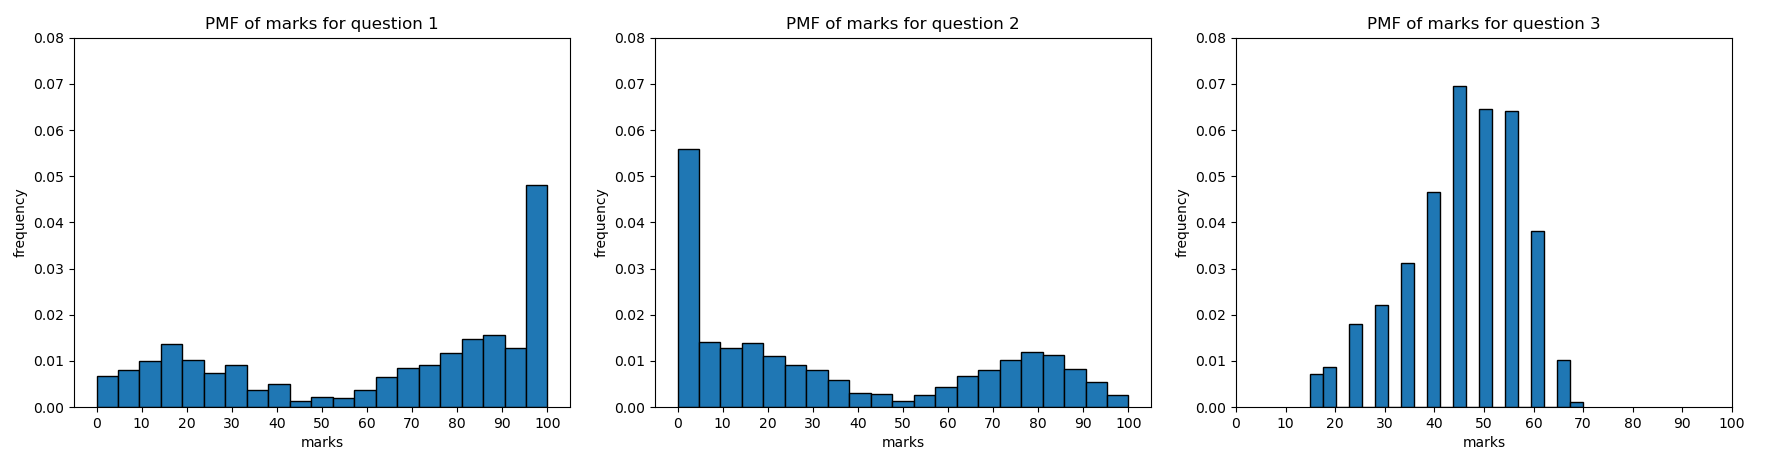
\includegraphics[scale=0.5]{q2_a.png}
\end{center}

From these graphs we might assume that the first question is the easiest because it has a large number of very high marks. We might also assume that the second question is the hardest because it has a large number of very low marks. It's difficult to assume anything about the final question as almost all of the marks are somewhat average with few high or low marks.

This approach gives us a rough estimate of how difficult the questions are relative to each other. However, this approach doesn't give us any indication of potential correlations between a student's marks for two different questions. Furthermore, this approach causes us to focus on the outlying marks, i.e., very high marks for the first question, without accounting for the mean or median marks.

\noindent (b) The \texttt{mark\_cond()} method from the code iterates over every student's results and keeps track of the question two and question three marks for each of the 21 possible question one marks. Then the method uses Python's built-in mean and variance methods to calculate the respective question two and question three values for each question 1 mark. It produces the following table of results:

\begin{center}
    \begin{tabular}{|c|cccc|c|cccc|}
        \hline
        $Q1$ & $\mu(Q2)$ & $\mu(Q3)$ & $var(Q2)$ & $var(Q3)$ & $Q1$ & $\mu(Q2)$ & $\mu(Q3)$ & $var(Q2)$ & $var(Q3)$ \\
        \hline
         0 & 0 & 22 & 0.0 & 38.5 & 55 & 12 & 47 & 50.0 & 50.0 \\
         5 & 0 & 27 & 0.7 & 58.2 & 60 & 12 & 46 & 33.0 & 37.7 \\
         10 & 0 & 30 & 1.0 & 53.7 & 65 & 13 & 46 & 54.6 & 38.7 \\
         15 & 1 & 33 & 5.6 & 50.6 & 70 & 17 & 47 & 58.7 & 34.6 \\
         20 & 2 & 36 & 9.2 & 65.6 & 75 & 20 & 49 & 46.5 & 40.9 \\
         25 & 2 & 39 & 21.1 & 42.8 & 80 & 29 & 51 & 135.0 & 36.2 \\
         30 & 6 & 40 & 39.4 & 46.2 & 85 & 40 & 50 & 323.8 & 40.0 \\
         35 & 6 & 42 & 43.8 & 47.8 & 90 & 60 & 50 & 382.5 & 34.9 \\
         40 & 7 & 44 & 23.2 & 36.9 & 95 & 60 & 53 & 374.1 & 39.7 \\ 
         45 & 8 & 44 & 26.7 & 54.2 & 100 & 82 & 55 & 105.6 & 43.8 \\
         50 & 12 & 44 & 50.3 & 41.4 & & & & & \\
         \hline
    \end{tabular}
\end{center}

Rather than use the binning ranges mentioned in the question statement I opted to stick with the original 21 bins from the data so as not to lose any detail or accuracy.

\noindent (c) Using the calculated mean and variance values from the previous question we can use the CLT ($\mu \pm 2\sigma/\sqrt{N}$) to find the 95\% confidence intervals for each question and mark. For each CI the value of $N$ depends on the number of marks in its respective bin. For each question one mark we can plot two bars (one for each of the other questions) and overlay an error bar representing the 95\% CI over each of them:

\begin{center}
    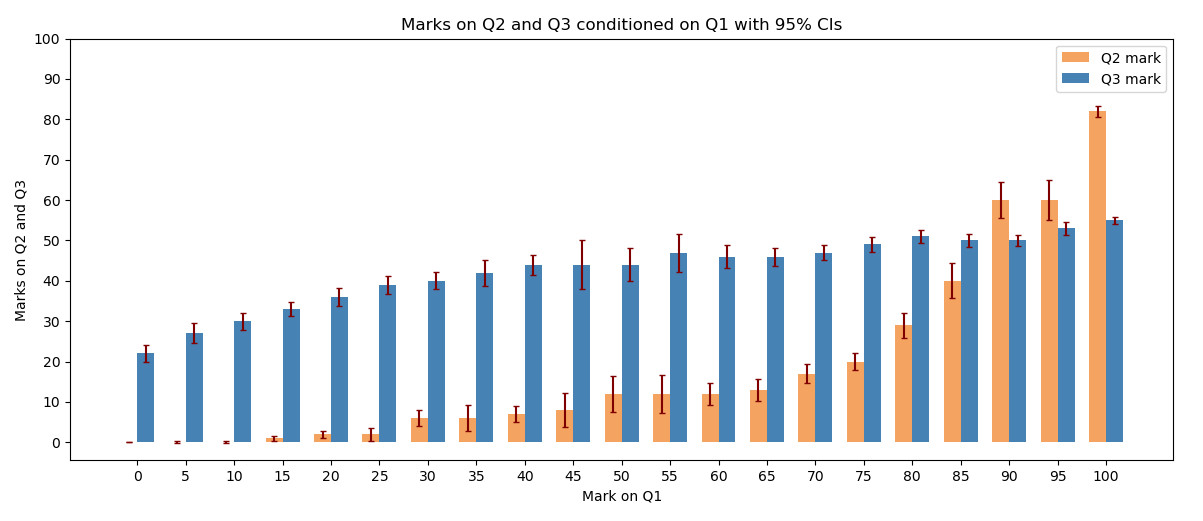
\includegraphics[scale=0.7]{q2_c.png}
\end{center}

From the above plot it definitely appears that question two is more difficult than question one given that, for every question one mark except zero, the question two mark is a great deal lower than the question one mark. This observation is also supported by the 95\% confidence intervals for the question two marks as they do not contain their respective question one marks either.

The third question is a little more complicated. When compared with the second question, it appears that question three is easier for all question one marks less than 90. This could, for example, be due to the particular nature of question three; perhaps the majority of the question is relatively easy but a certain section is very difficult leading to few very high marks.

When comparing the relative difficulty of question three with question one we notice another interesting phenomenon: low scorers in question one receive much higher relative marks in question three while high scorers in question one receive much lower relative marks in question three. Again, this could be due to the nature of question three. We can conclude that it is very easy to receive some marks in question three but extremely difficult to achieve high marks. This could tell us that question three ought to be rebalanced or changed somewhat.

\noindent (d) We can use linear regression to predict a student's mark for another question, e.g. question two, given their mark for question one. We can use the marks for question one and two from our dataset as the training data where the $i^{th}$ mark for question one is our input, $x^{(i)}$, and the $i^{th}$ mark for question two is our output, $y^{(i)}$. We need to find parameters, $\theta_0$ and $\theta_1$, such that $y^{(i)}$ is close to $h_{\theta}(x^{(i)}) = \theta_0 + \theta_1 x^{(i)}$ for all of the training data. To do this we can use the least squares method to minimise the a cost function like so: $J(\theta_0, \theta_1) = \frac{1}{m} \sum_{i=1}^m \left( h_{\theta}(x^{(i)}) - y^{(i)} \right)^2$, where $m$ is the number of items in our training data. Once we've found suitable parameters we can pass the question one mark into our function $h_{\theta}(x)$ and predict the corresponding mark for question two.

Based on the calculations from the two previous questions it would appear that our assumption that the mean (of the question two/three marks) was a linear function of the feature (the question one mark) was, in fact, appropriate. We can estimate this using the plot from part (c): for both questions two and three their respective relationships with the marks in question one are quite linear. Other than a slight curve upwards in the line for question two towards the end the relationships appear entirely linear.

With linear regression randomness is introduced through the errors or differences between the line $y = h_{\theta}(x)$ and the actual values themselves. We assume that these errors are normally distributed within our model. Judging by our plotted confidence intervals from (c) it would appear that most of the exam marks fall fairly close to the calculated means which would lead us to believe that our use of linear regression is appropriate, in this case.

\noindent (e) Given that the marks are normally distributed about the mean, $X_{ij}$, we can use the standard expression for the PDF of a Gaussian random variable like so:

$$P(X_{ij} = x \mid S_i, D_j) = \frac{1}{\sqrt{2\pi}} e^{-\frac{(x - (S_i - D_j))^2}{2}}$$

We can then calculate the log-likelihood of the dataset by getting the log of the product of the PDFs for all $i = 1, \cdots, 1000$ students and all $j = 1, 2, 3$ questions:

$$\log \left( \prod_{i=1}^{1000} \prod_{j=1}^3 \frac{1}{\sqrt{2\pi}} e^{-\frac{(x^{(i)(j)} - (S_i - D_j))^2}{2}} \right)$$
$$= \sum_{i=1}^{1000} \sum_{j=1}^3 \log \left( \frac{1}{\sqrt{2\pi}} e^{-\frac{(x^{(i)(j)} - (S_i - D_j))^2}{2}} \right)$$
$$=- \log \left( \frac{1}{2\sqrt{2\pi}^{3000}} \right) \sum_{i=1}^{1000} \sum_{j=1}^{3} (x^{(i)(j)} - (S_i - D_j))^2$$

\noindent (f) We can use the expression for the log-likelihood of the dataset that we previously found as our cost function and can iteratively modify our parameters $S_i$ and $D_j$ to minimise its value. We begin by randomly selecting starting values for our parameters and, given some learning rate $\alpha$, we can run the standard gradient descent algorithm until we've successfully reach the minimum. This will provide us with the maximum likelihood estimates of our parameters $S_i$ and $D_j$.

\section*{Appendix: Code}

\subsection*{Question 1}

\begin{lstlisting}[language=Python]
import matplotlib.pyplot as plt
import numpy as np
from math import sqrt
from random import choice, sample
from scipy.special import comb

# Questions 1 (c) and 1 (d)
def plot_prob(n, p):    
    plt.plot(n, p, 'r')
    plt.xlabel(r'$n$')
    plt.ylabel('Probability')
    plt.title(r'Probability of failing having studied $n$ topics')
    plt.xticks(np.arange(0, 11, 1))
    plt.yticks(np.arange(0, 1.1, 0.1))
    plt.show()

n = np.linspace(0, 10, 11)

# Question 1 (c)
p1 = (comb(10 - n, 3) + (comb(10 - n, 2) * n)) / 120
plot_prob(n, p1)

# Question 1 (d)
p2 = (comb(10 - n, 4) + (comb(10 - n, 3) * n)) / 210
plot_prob(n, p2)

# Question 1 (e)
def sim_e(n):
    topics = list(range(10))
    studied = set(sample(topics, n))
    exam = set(sample(topics, 3))
    return 1 if len(exam & studied) >= 2 else 0

# Question 1 (f)
def sim_f(n, N):
    mean = sum(sim_e(n) for _ in range(N)) / N
    var = mean * (1 - mean)
    ci = (mean - 2 * sqrt(var / N), mean + 2 * sqrt(var / N))
    return mean, var, ci

print(sim_f(7, 1000))
print(sim_f(7, 10000))

# Question 1 (g)
def sim_g(n, N, sims):
    lo, hi = sim_f(n, N)[2]
    means = [sim_f(n, N)[0] for _ in range(sims)]
    count = sum(map(lambda mean: mean >= lo and mean <= hi, means))
    return count / sims

print(sim_g(7, 1000, 500))
print(sim_g(7, 10000, 500))

# Question 1 (h)
def sim_h(n, N, change):
    passes = 0
    for _ in range(N):
        # assume topics 0, 1, 2 were on previous exam
        if change < 0:
            studied = set(list(range(10))[-n:])
            biased = list(range(3, 10))
        else:
            studied = set(range(n))
            biased = list(range(3))
        topics = list(range(10))
        for topic in biased:
            topics.extend([topic] * abs(change))
        exam = set([])
        while len(exam) != 3:
            exam.add(choice(topics))
        passes += 1 if len(exam & studied) >= 2 else 0
    return passes / N

for change in range(-5, 6):
    print(change, sim_h(5, 10000, change))
\end{lstlisting}

\subsection*{Question 2}

\begin{lstlisting}[language=Python]
import matplotlib.pyplot as plt
import numpy as np
from math import sqrt
from statistics import mean, variance

# Dataset
def parse_marks():
    return tuple(zip(*[list(map(int, line.strip().split())) \
        for line in open("dataset.txt").readlines()[1:]]))

marks = parse_marks()

# Question 2 (a)
def pmf_hist(marks, question):
    plt.hist(marks[question], 21, density=True, edgecolor='black')
    plt.xlabel('marks')
    plt.ylabel('frequency')
    plt.title(f'PMF of marks for question {question + 1}')
    plt.xticks(np.arange(0, 110, 10))
    plt.yticks(np.arange(0, 0.09, 0.01))
    plt.show()

for question in range(3):
    pmf_hist(marks, question)

# Question 2 (b)
def mark_cond(marks):
    q1_marks = {}
    for i in range(1000):
        q1, q2, q3 = marks[0][i], marks[1][i], marks[2][i]
        if q1 not in q1_marks:
            q1_marks[q1] = [[], []]
        q1_marks[q1][0].append(q2)
        q1_marks[q1][1].append(q3)
    data = {}
    for mark in q1_marks:
        mean_q2 = int(round(mean(q1_marks[mark][0])))
        mean_q3 = int(round(mean(q1_marks[mark][1])))
        var_q2 = variance(q1_marks[mark][0])
        var_q3 = variance(q1_marks[mark][1])
        data[mark] = (mean_q2, var_q2, mean_q3, var_q3, len(q1_marks[mark][0]),
            len(q1_marks[mark][1]))
    return data

cond_data = mark_cond(marks)
for mark in cond_data:
    cond_datum = cond_data[mark]
    print(
        'q1_mark=%d, mean_q2=%d, var_q2=%.2f, mean_q3=%d, var_q3=%.2f' %
        (mark, cond_datum[0], cond_datum[1], cond_datum[2], cond_datum[3])
    )

# Question 2 (c)
def mark_cond_conf(marks):
    cond_data = mark_cond(marks)
    labels = list(map(str, range(0, 105, 5)))
    q2_marks = [cond_data[mark][0] for mark in sorted(cond_data)]
    q3_marks = [cond_data[mark][2] for mark in sorted(cond_data)]
    q2_clts = [
        2 * sqrt(cond_data[mark][1]) / sqrt(cond_data[mark][4])
        for mark in sorted(cond_data)
    ]
    q3_clts = [
        2 * sqrt(cond_data[mark][3]) / sqrt(cond_data[mark][5])
        for mark in sorted(cond_data)
    ]
    x, w = np.arange(len(labels)), 0.35
    fig, ax = plt.subplots()
    ax.bar(x - w / 2, q2_marks, w, label='Q2 mark', color='sandybrown', yerr=q2_clts,
        ecolor='maroon', capsize=2)
    ax.bar(x + w / 2, q3_marks, w, label='Q3 mark', color='steelblue', yerr=q3_clts,
        ecolor='maroon', capsize=2)
    ax.set_xlabel('Mark on Q1')
    ax.set_ylabel('Marks on Q2 and Q3')
    ax.set_title('Marks on Q2 and Q3 conditioned on Q1 with 95% CIs')
    ax.set_xticks(x)
    ax.set_xticklabels(labels)
    ax.set_yticks(np.arange(0, 110, 10))
    ax.legend()
    fig.tight_layout()
    plt.show()

mark_cond_conf(marks)
\end{lstlisting}

\end{document}
